\section[Requirements]{Requirements}
\label{section:requirements}



% help site at http://www.projectmanagementhelp.com/how-to-write-functional-requirements/
% bullet point these requirements, describe them, specify any details.
% include bain quite as footnote
\subsection{Functional Requirements}

% what it is 
% what it will be used for
% how we will measure success

The game will be a real-time strategy game set in space. Opposing fleets of spacecraft
will battle each other. A player's goal is to ensure the survival of their fleet and the destruction
of the enemy.

\begin{description}

	\item[Multiplayer]

	As a multiplayer game, two players must be able to participate in a battle against each other.
	These players will be on different computers on the same network. The game must be capable of running
	smoothly on a local area network, which experiences less disruption than the Internet. To this end, a client server model will be used.

	\item[Fleets]

	Each player will control a fleet of ships. Ships have two health stats: hull and shields. Once hull health has been reduced to zero then the ship is destroyed. However, functioning shields prevent hull damage. It is intended that shields be relatively fast to recharge but hull damage is slow and expensive to repair.

	\item[Ship Customisation]

	The ships that make up a player's fleet will each have a number of pluggable slots. Prior to a game each player will be able to customise the ships in their fleet by filling these slots with different pieces of equipment. There will be two types of slot: system slots and weapons slots, the latter also split into the areas on the ship it can be installed on. System slots allow for extra internal systems to be added to the ship, for example extra shields or long range scanners. Weapons slots allow the player to choose which types of weapons their ships will use; however, a fleet budget will prevent a user from using the best weapons on every ship. See figure \ref{fig:ship_design}.

\begin{marginfigure}
	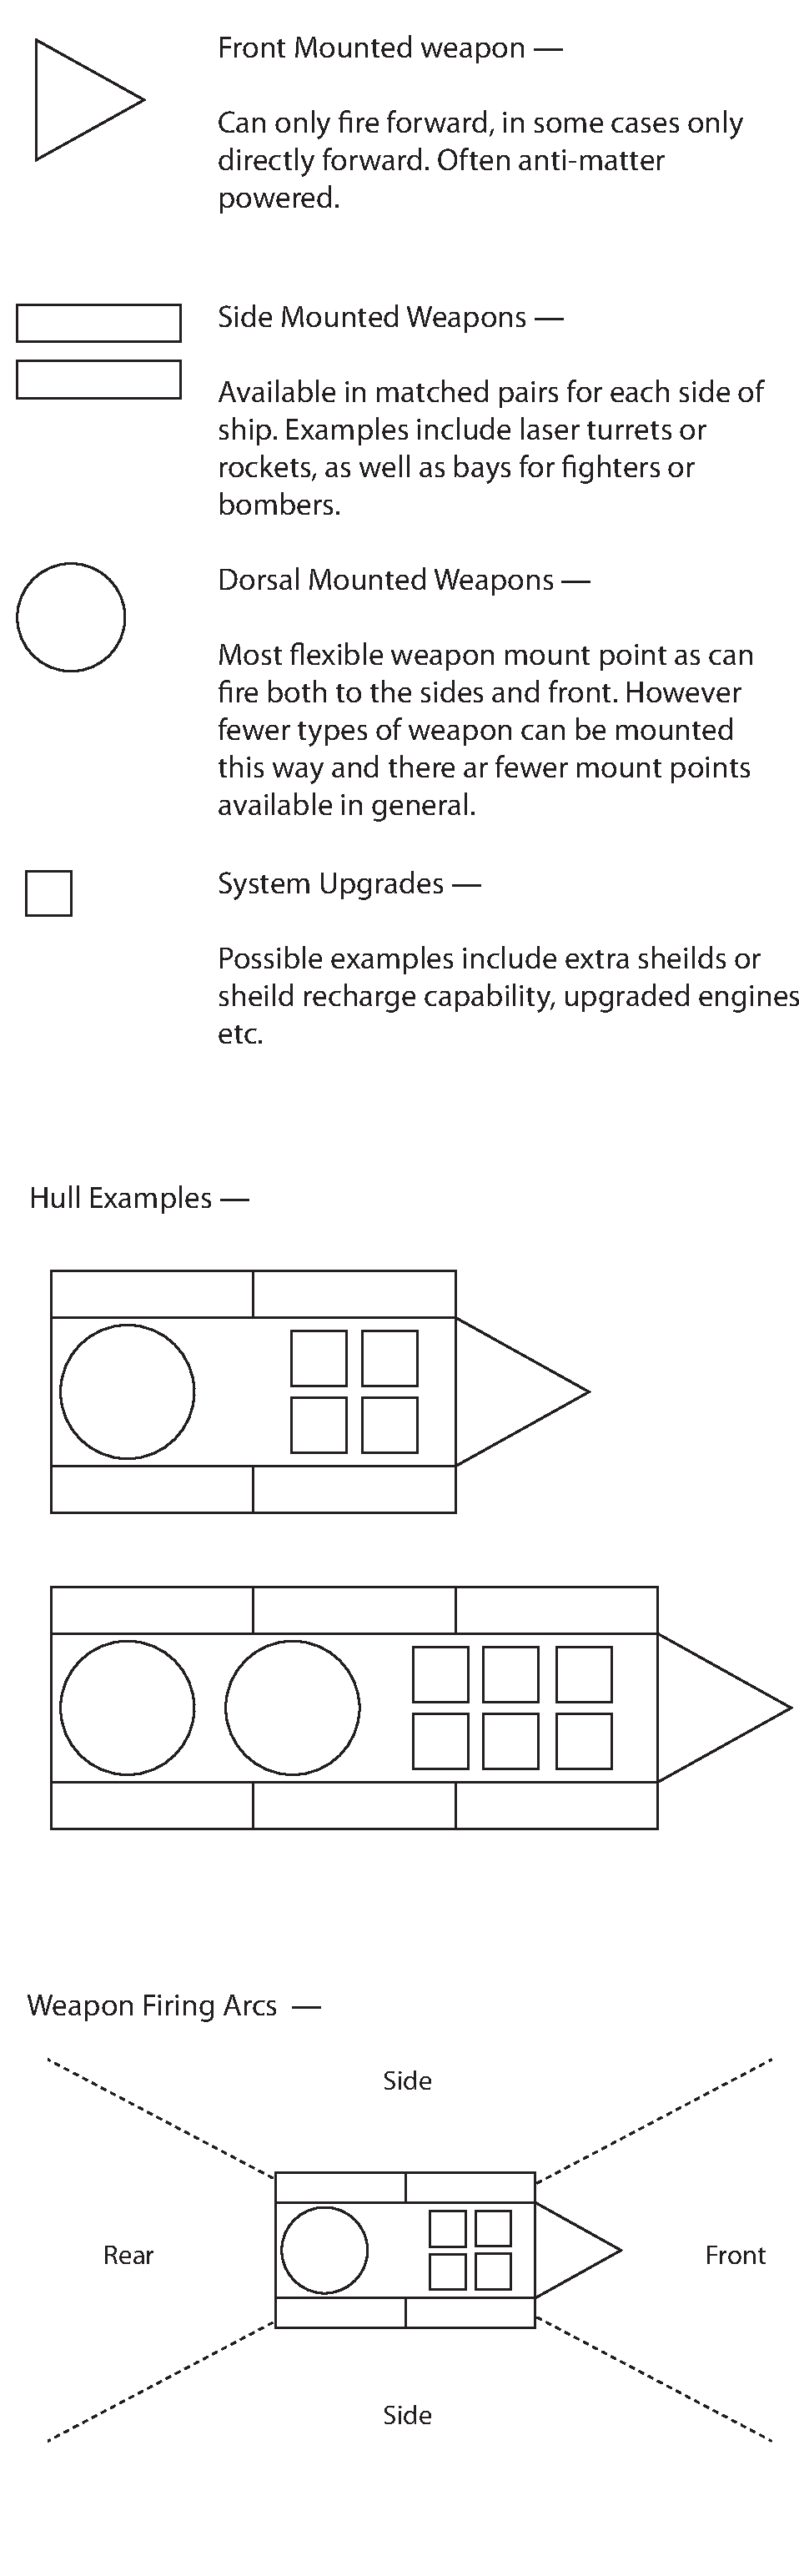
\includegraphics[width=6cm]{res/ship_design}
	\caption{Diagrams showing basic conception of ship customisation and weapon configurations. }
	\label{fig:ship_design}
\end{marginfigure}


	\item[Resource System]

	Three resources exist within the game: fuel, metal, and anti-matter. These resources are only used by the ships. Fuel maintains a ship's shields, without a shield any damage will be done to the ship's hull. Metal is used to slowly repair a ship's hull after it has been damaged. Anti-matter is a rare resource that is used by the more powerful weapons available.

	Planets generate a constant supply of resources, so players can gain extra resources via planetary capture. The resources generated by the planets owned by a player feed into that player's global stockpile. Individual ships then draw resources from this stockpile.

	% Do ships get resources from the stockpile automatically, or do they have to visit planets?

	\item[Planetary Capture]

	Planet ownership is the only method of generating resources. Planets can only belong to
	one player at a time at most. To capture a planet, a player must have their ships in control
	of the planet for a certain period of time. If the planet belongs to the enemy then it will
	take twice as long for it to be captured than an unoccupied planet.

	% \item[Tactical Zoom]

	\item[Fog of War]

	Players must not be able to see the state of the entire map unless they control it all. There
	will be three levels to the fog of war: unknown, visited, and visible. Any locations on the map
	that a player's ships have not visited will be `unknown' and the player will not be able to see
	anything that is at that location. Any locations that have been explored at least once will be
	`visited'; the player will be able to see the general layout of the area, but not any details
	such as enemy ships. Finally, any locations covered by planets or ships owned by the player will
	be `visible' and all aspects of the map in the area will be revealed to the player.
	
	\item[AI]

	A sophisticated artificial intelligence system will be an important component in the game.
	Each player's fleet will be controlled through an AI system. It will use a planning algorithm
	that takes a high level objective given by the player and generates a series of steps to
	achieve that objective. The AI must control the individual ships that make up the fleet; it
	is up to the human player to decide on the overall strategy of the fleet.

	A successful AI system must receive orders and quickly convert them into a sensible series of
	actions which it performs autonomously. If an impossible goal is set, or an existing goal is
	invalidated by changes to the world, then the AI must detect this and stop acting on it.

	% Basic AI elements, e.g. pathfinding

	\item[Campaign]

	A campaign mode will be available which consists of a fixed number of battles between the two players.
	The final battle will be the `showdown' that determines the overall winner. The victor of each of
	the earlier battles will be granted bonuses toward the final battle, giving them an advantage against
	their opponent.

	Between every battle each player will have an opportunity to perform minor customisations on
	the ships in their fleet.

	\item[Operating System Requirements]

	The game must be playable on recent versions of Mac OS X and Linux. The nature of the libraries that are likely to be used for development make it possible that also supporting Windows will be relatively easy, but this is not guaranteed and no commitment on it is being made at this stage.

% \item[Gameplay]
% mention ship destruction and resources that drained during battle, not loss of ships

\end{description}

\subsection{Non-Functional Requirements}

\begin{description}

	\item[Fun]

	One of the most important requirements is that the game should be fun to play. Players should enjoy the game and want to play it multiple times.

	\item[Short game sessions]

	An individual battle should not last too long. If a game is likely to take a number of hours it is a barrier to entry for players as they must schedule large amounts of their time if they are to play at all. The aim should be for an individual battle to last between 20 and 35 minutes. Tournaments or campaigns are possible optional features that could extend this to provide inbuilt support for longer playing sessions.

	\item[Reliable]

	Both the client and server should be stable programs that are not prone to crashing. If either were to crash regularly then it would ruin the experience and cause people to stop playing the game.

	The networking component should also be reliable. Minor network disruption should not cause a huge loss in communication between the clients and server.

	\item[Secure] 
	
	Although the game server will initially be intended for LAN usage it is important that it should not cause a computer running it on the Internet to be exploitable. It should not be vulnerable to attacks such as denial of service, which would stop the machine from performing any other tasks whilst under attack, or remote code execution, which could allow an attacker to take control of the target machine. 
	
	Furthermore, the game system should be proof against cheating by modification of the client code or packet injection attacks, or other similar methods of gaining an unfair advantage. 

	% Macromanagement?

\end{description}

